\documentclass[12pt]{article}
\usepackage{amsmath}
\usepackage{graphicx}
\usepackage{caption}

\begin{document}

\title{GCP Error Log vs RP Frequency Analysis}
\date{8/5/2015}
\author{Alex Zahn}

\maketitle

\section{Motivation}

GCP debug logs from the first round of factory acceptance testing indicate two easily identifiable failure modes during track beam mode.

The first issue is that GCP attempts to order the ACB in and out of track beam mode many times before finally leaving it in track beam mode, and operating mostly normally (see below). During this ``initialization" period, we see many skipped header indices and very few responses from the ACB. Additionally, GCP logs many spurious interrupt errors. Typically this occurs for the first three to ten seconds of operation.

The second issue is that after the traumatic initialization period, both GCP and the ACB appear to repeat messages at each other several times before proceeding to the next header index. Skipped header indices stop appearing, however.

One theory is that the GCP test machine was not properly syncing to the RP signal, and could have significant nondeterministic latency between receiving an RP edge and sending a track beam command. If true, this would result in RP intervals during which an unknown number of track beam mode commands get sent to the ACB. Considering the slowness of the RS232 and RS422 protocols, it is very possible that some track beam commands may actually straddle an RP edge. It may also be possible that GCP is being preempted mid operation, separately contributing to nondeterministic latency.

Since the interface specification states that the ACB is a hard real time system that expects exactly one track beam mode command per RP interval, we do not currently know how the ACB would (or even should) respond to a situation like this. 

To test this theory, we lowered the RP frequency from pb1's 95 Hz to 80 Hz and 59 Hz, collecting GCP debug logs from track beam mode operation at all three frequencies. The idea is that in the limit that the RP interval becomes very long, the variance in the GCP test machine's latency becomes negligible, and resend events should become rare.

\section{Log Contents}

The GCP debug logs record the track beam mode commands sent to the ACB, and the responses received from the ACB in time order. The logs also contain some internal error messages generated by GCP.

\subsection{Send/Receive Format}

An example line recording a track beam command is 
\begin{center}
\texttt{sending 0.560256sec 50 58 0 36 0 0 0 0 1 0 0 0 0 0 0 3f}
\end{center}
The response lines are very similar:
\begin{center}
\texttt{receiving 0.667555sec 50 58 3 34 4 35 4 3b c0 e9 3b 2e 30 e e2 0 57 0 0 0 53 0 0 0 0 0 0 0 0 0 0 0 0 0 0 0 0 0 0 0 0 0 0 0 0 0 0 d5 }
\end{center}

The actual packet that went over the serial port starts after the time stamp. Each packet begins with 5058 (an ascii PX) and is formatted so that each space delimited character or pair of characters is the hex value of a single byte.

The byte ordering and content of the responses is likely to change soon, though command format is almost certainly frozen in. For our purpose here though, it is only relevant that the first two bytes following the PX represent the header value.

Importantly, each command and response is supposed (and expected by both GCP and the ACB) to increment over the previous command or response, and the header values of responses and commands belonging to the same RP interval should be equal. Essentially our experiment described in this document is dedicated to identifying any deviation from this specified behavior.

\subsection{Errors logged by GCP}

The debug logs contain many different types of messages (some indicating errors, some not) recording GCP's activity, especially when attempting to first place the ACB in track beam mode. I watched only two of these messages.

The first is the spurious interrupt error. These occur when the GCP process responsible for reading the ACB response or sending an ACB command detects that it has been woken up too early or too late for the next RP interval, based on the system clock. In normal operation, the sptAntennaControl process is supposed to have an interrupt handler registered on a parallel port RP edge that should guarantee that the relevant ACB command and receive code runs exactly once per RP interval, hopefully near the beginning of the interval so as to leave enough time to complete the send/receive cycle before the next interval starts.

The second is the invalid sequence response error. This occurs when GCP detects a header value mismatch between a command and response (is this correct?). When GCP throws this error, it will attempt to make the ACB exit and re-enter track beam mode. 

\section{Results}

We actually do find that lowering the RP frequency helps the resend issue significantly.

The crudest way to demonstrate this is to just count the density of spurious interrupt and invalid sequence response errors per line of log file. Ideally, we could find the number of errors per time in units of RP periods, but the log does not seem to be giving the real system time; the time field in the sending and receiving lines seems to roll over a little faster than once per second.

\begin{center}

Errors per Line \linebreak

\begin{tabular}{cccc}
  & 95 Hz & 80 Hz & 59 Hz \\ 
spurious interrupt & 0.11 & 0.04 & 0.03 \\ 
invalid sequence response & 0.10 & 0.002 & 0.002 \\ 
\end{tabular} 
\end{center}

In a ``correct" log file, we would only ever alternating and receiving lines. Instead, we see many command and response repetitions. We can visualize this by taking the discrete derivative of the sequence of line numbers at which commands or responses appear. Any value that is higher than two represents repetitions of something else (almost always a response), and any value lower than two represents a repetition of the command. Note that we don't account for skipped indices, because they don't seem to happen after initialization.

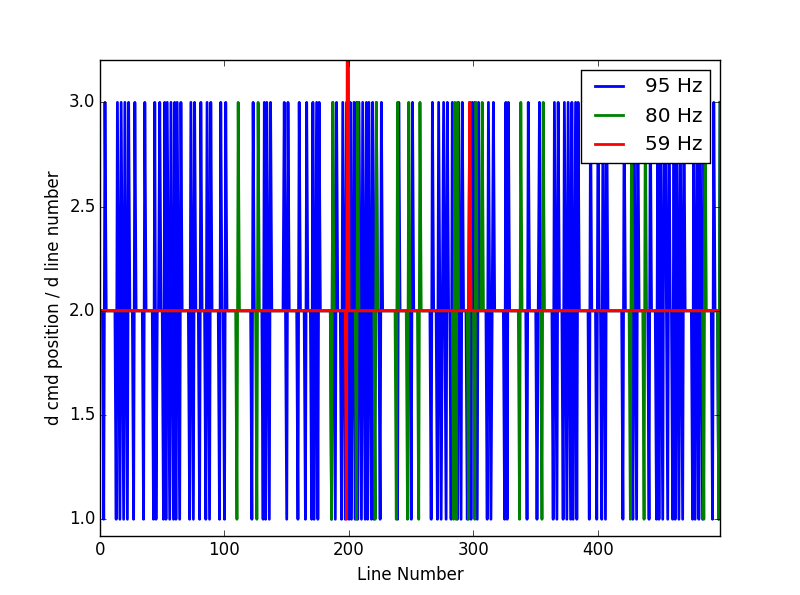
\includegraphics[scale=.7]{cmd_lno_all.png}
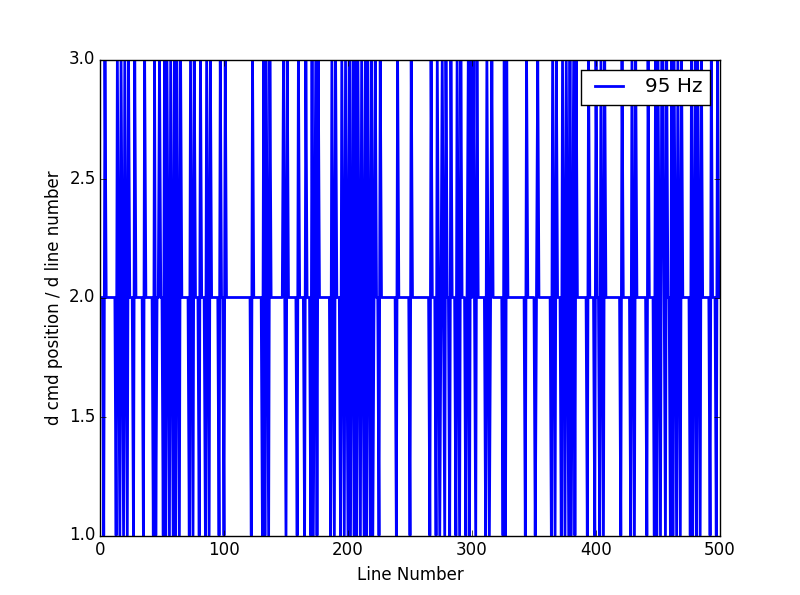
\includegraphics[scale=.7]{cmd_lno_95.png}
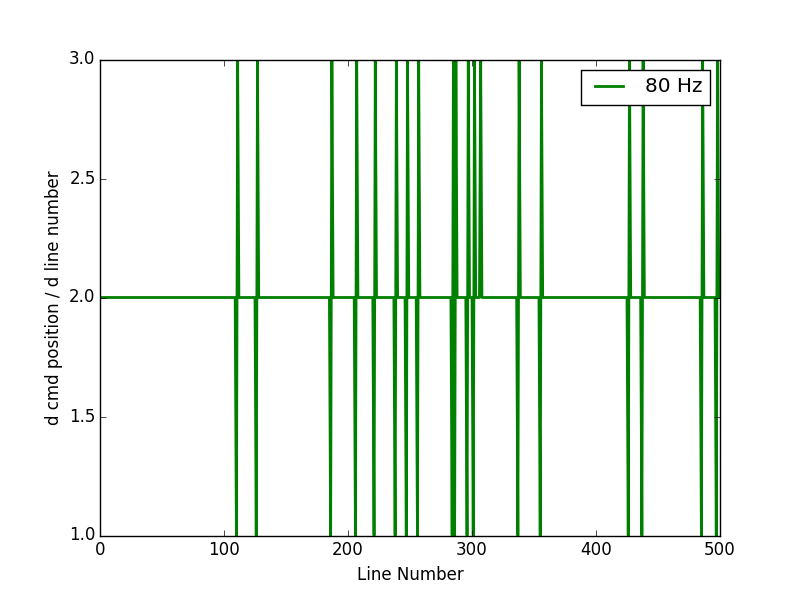
\includegraphics[scale=.7]{cmd_lno_80.png}
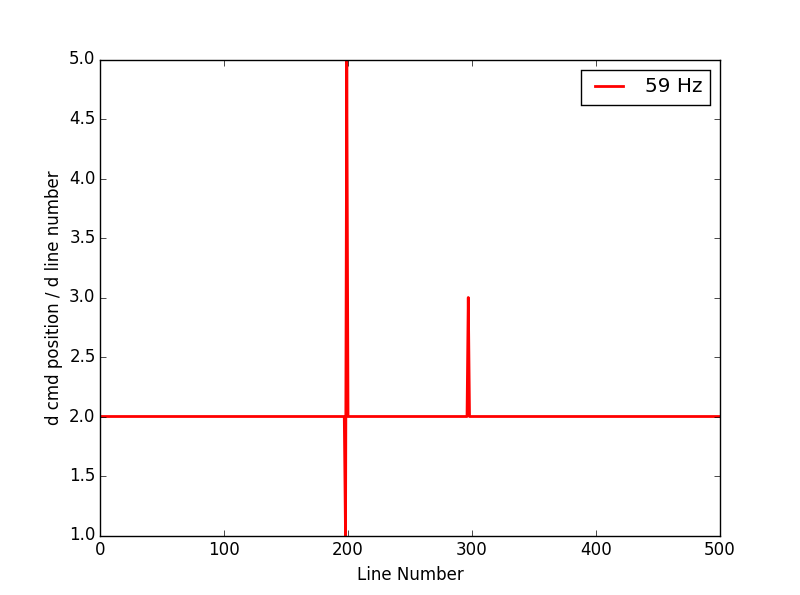
\includegraphics[scale=.7]{cmd_lno_59.png}

The corresponding graphs for command repetitions show the same behavior.

To be slightly more quantitative, the fraction of logged resent commands at 95 Hz is 0.17, with a resent response rate of 0.18. At 59 Hz, this falls to 0.004 and 0.003, respectively.


\end{document}